\documentclass[12pt,a4paper,oneside]{report}

%--------------------------------------------------------------------
% PAGE GEOMETRY
%--------------------------------------------------------------------
\usepackage[a4paper, top=1in, bottom=1in, left=1.25in, right=1in, headheight=15pt, headsep=15pt, footskip=25pt]{geometry}

%--------------------------------------------------------------------
% FONT: Times New Roman equivalent
%--------------------------------------------------------------------
\usepackage{newtxtext}
\usepackage{newtxmath}

%--------------------------------------------------------------------
% CORE PACKAGES
%--------------------------------------------------------------------
\usepackage{graphicx}
\usepackage{float}
\graphicspath{{./}{../code/}{../diagrams/}{diagrams/}}
\usepackage{setspace}
\usepackage{parskip}
\usepackage{booktabs}
\usepackage{tabularx}
\usepackage{array}
\usepackage{enumitem}
\usepackage{indentfirst}
\usepackage{microtype}
\usepackage{fancyhdr}
\usepackage{titlesec}
\usepackage{tocloft}
\usepackage{hyperref}

\hypersetup{
  colorlinks=false,
  pdfborder={0 0 0},
  pdftitle={Ledger: AI-Based Fake News Detection System},
  pdfauthor={Group 12, CEC}
}

%--------------------------------------------------------------------
% LINE SPACING
%--------------------------------------------------------------------
\setstretch{1.5}

%--------------------------------------------------------------------
% PARAGRAPH INDENT / SKIP
%--------------------------------------------------------------------
\setlength{\parindent}{0.5in}
\setlength{\parskip}{0pt}

%--------------------------------------------------------------------
% CHAPTER / SECTION TITLE FORMATTING  (mirrors the sample PDFs)
%--------------------------------------------------------------------
\titleformat{\chapter}[display]
  {\normalfont\bfseries\centering}
  {\large Chapter \thechapter}
  {0pt}
  {\Large\MakeUppercase}
\titlespacing*{\chapter}{0pt}{0pt}{24pt}

\titleformat{\section}
  {\normalfont\large\bfseries}
  {\thesection}
  {1em}{}
\titlespacing*{\section}{0pt}{18pt}{6pt}

\titleformat{\subsection}
  {\normalfont\normalsize\bfseries}
  {\thesubsection}
  {1em}{}
\titlespacing*{\subsection}{0pt}{12pt}{4pt}

%--------------------------------------------------------------------
% HEADERS AND FOOTERS
%--------------------------------------------------------------------
\pagestyle{fancy}
\fancyhf{}
\fancyhead[L]{\small College of Engineering, Cherthala}
\fancyhead[R]{\small\nouppercase{\leftmark}}
\fancyfoot[L]{\small Department of Computer Science and Engineering}
\fancyfoot[R]{\small\thepage}
\renewcommand{\headrulewidth}{0.4pt}
\renewcommand{\footrulewidth}{0.4pt}

% Default plain style in front matter (centered roman page numbers, no header, no rule)
\fancypagestyle{plain}{
  \fancyhf{}
  \fancyfoot[C]{\small\thepage}
  \renewcommand{\headrulewidth}{0pt}
  \renewcommand{\footrulewidth}{0pt}
}

% Front-matter style (centered roman page numbers, no header, no rule)
\fancypagestyle{frontmatter}{
  \fancyhf{}
  \fancyfoot[C]{\small\thepage}
  \renewcommand{\headrulewidth}{0pt}
  \renewcommand{\footrulewidth}{0pt}
}

\renewcommand{\chaptermark}[1]{\markboth{#1}{}}

%--------------------------------------------------------------------
% TOC appearance
%--------------------------------------------------------------------
\renewcommand{\cftchapleader}{\cftdotfill{\cftdotsep}}
\renewcommand{\cftsecleader}{\cftdotfill{\cftdotsep}}
\renewcommand{\cftfigleader}{\cftdotfill{\cftdotsep}}

%====================================================================
\begin{document}
%====================================================================

% ===================================================================
% COVER PAGE
% ===================================================================
\begin{titlepage}
\thispagestyle{empty}
\begin{singlespace}
\centering
\vspace*{0.3cm}

{\large\bfseries MAJOR PROJECT REPORT}\\[0.1cm]
{\large\bfseries ON}\\[0.5cm]

{\Large\bfseries Ledger: AI-Based Fake News Detection System}\\[0.25cm]
{\Large\bfseries Using Explainable AI}\\[0.7cm]

{\normalsize\itshape Submitted By}\\[0.25cm]
{\normalsize\bfseries ANANDHAKRISHNAN S (CEC23CS033)}\\[0.1cm]
{\normalsize\bfseries ARAVIND A KAMATH (CEC23CS041)}\\[0.1cm]
{\normalsize\bfseries ARJUN MANOJ (CEC23CS043)}\\[0.1cm]
{\normalsize\bfseries SANGEETH KRISHNAN S (CEC23CS105)}\\[0.6cm]

{\normalsize\itshape under the esteemed guidance of}\\[0.2cm]
{\normalsize\bfseries Mrs. Rajeswary R}\\[0.1cm]
{\normalsize Assistant Professor}\\[0.1cm]
{\normalsize Department of Computer Science and Engineering}\\[0.7cm]


\includegraphics[width=3.2cm]{CEC_Logo.jpeg}\\[0.5cm]

{\normalsize\bfseries SEPTEMBER 2026}\\[0.15cm]
{\normalsize\bfseries DEPARTMENT OF COMPUTER SCIENCE AND ENGINEERING}\\[0.08cm]
{\normalsize\bfseries COLLEGE OF ENGINEERING, PALLIPPURAM P O, CHERTHALA,}\\[0.08cm]
{\normalsize\bfseries ALAPPUZHA PIN: 688541,}\\[0.08cm]
{\normalsize PHONE: 0478 2553416, FAX: 0478 2552714}\\[0.04cm]
{\normalsize http://www.cectl.ac.in}
\end{singlespace}
\end{titlepage}

% ===================================================================
% INNER TITLE PAGE
% ===================================================================
\begin{titlepage}
\thispagestyle{empty}
\begin{singlespace}
\centering
\vspace*{0.3cm}

{\large\bfseries MAJOR PROJECT REPORT ON}\\[0.5cm]

{\Large\bfseries Ledger: AI-Based Fake News Detection System}\\[0.25cm]
{\Large\bfseries Using Explainable AI}\\[0.7cm]

{\normalsize\itshape Submitted By}\\[0.25cm]
{\normalsize\bfseries ANANDHAKRISHNAN S (CEC23CS033)}\\[0.1cm]
{\normalsize\bfseries ARAVIND A KAMATH (CEC23CS041)}\\[0.1cm]
{\normalsize\bfseries ARJUN MANOJ (CEC23CS043)}\\[0.1cm]
{\normalsize\bfseries SANGEETH KRISHNAN S (CEC23CS105)}\\[0.5cm]

{\normalsize\itshape under the esteemed guidance of}\\[0.2cm]
{\normalsize\bfseries Mrs. Rajeswary R}\\[0.5cm]

{\normalsize In partial fulfillment of the requirements for the award of the degree of}\\[0.2cm]
{\normalsize\bfseries Bachelor of Technology}\\[0.1cm]
{\normalsize in}\\[0.1cm]
{\normalsize\bfseries Computer Science and Engineering}\\[0.1cm]
{\normalsize of}\\[0.1cm]
{\normalsize\bfseries APJ Abdul Kalam Technological University}\\[0.65cm]


\includegraphics[width=3cm]{CEC_Logo.jpeg}\\[0.5cm]

{\normalsize\bfseries SEPTEMBER 2026}\\[0.15cm]
{\normalsize\bfseries DEPARTMENT OF COMPUTER SCIENCE AND ENGINEERING}\\[0.08cm]
{\normalsize\bfseries COLLEGE OF ENGINEERING, PALLIPPURAM P O, CHERTHALA,}\\[0.08cm]
{\normalsize\bfseries ALAPPUZHA PIN: 688541,}\\[0.08cm]
{\normalsize PHONE: 0478 2553416, FAX: 0478 2552714}\\[0.04cm]
{\normalsize http://www.cectl.ac.in}
\end{singlespace}
\end{titlepage}

% ===================================================================
% CERTIFICATE
% ===================================================================
\clearpage
\thispagestyle{empty}

\begin{center}
{\large\bfseries DEPARTMENT OF COMPUTER SCIENCE AND ENGINEERING}\\[0.15cm]
{\large\bfseries COLLEGE OF ENGINEERING CHERTHALA}\\[0.15cm]
{\large\bfseries ALAPPUZHA-688541}\\[0.6cm]

\includegraphics[width=2.8cm]{CEC_Logo.jpeg}\\[0.6cm]
{\Large\bfseries C E R T I F I C A T E}\\[0.7cm]
\end{center}

\noindent This is to certify that, the project report titled \textbf{LEDGER: AI-BASED FAKE NEWS
DETECTION SYSTEM USING EXPLAINABLE AI}, is a bonafide record of the CSD 415 Project
Phase I presented by \textbf{ANANDHAKRISHNAN S} (Reg.\,No. CEC23CS033),
\textbf{ARAVIND A KAMATH} (Reg.\,No. CEC23CS041), \textbf{ARJUN MANOJ}
(Reg.\,No. CEC23CS043), \textbf{SANGEETH KRISHNAN S} (Reg.\,No. CEC23CS105),
Seventh Semester B.\,Tech. Computer Science and Engineering students, under our guidance
and supervision, in partial fulfillment of the requirements for the award of the degree,
B.\,Tech. Computer Science and Engineering of APJ Abdul Kalam Technological University.

\vspace{3.5cm}

\noindent
\begin{tabular*}{\textwidth}{@{}p{0.33\textwidth}p{0.33\textwidth}p{0.33\textwidth}@{}}
  \textbf{Guide} & \textbf{Co-ordinator} & \textbf{HOD}\\[0.2cm]
  \textbf{Mrs. Rajeswary R} & \textbf{Mrs. Rakhi R} & \textbf{Dr. Preetha Theresa Joy}\\
  Assistant Professor & Assistant Professor & Professor\\
  Dept. of Computer Science & Dept. of Computer Science & Dept. of Computer Science\\
  \& Engineering & \& Engineering & \& Engineering
\end{tabular*}

% ===================================================================
% ACKNOWLEDGEMENT
% ===================================================================
\clearpage
\pagestyle{frontmatter}
\pagenumbering{roman}
\setcounter{page}{1}

\begin{center}
{\Large\bfseries ACKNOWLEDGEMENT}
\end{center}
\vspace{0.5cm}

This work would not have been possible without the support of many people.
First and foremost, we give thanks to Almighty God who gave us the inner strength,
resource and ability to complete our project successfully.

We would like to thank \textbf{Dr. Jaya V.L}, our Principal, who has provided us with
the best facilities and atmosphere for the project completion and presentation.
We would also like to thank our HOD \textbf{Dr. Preetha Theresa Joy} (Professor,
Department of Computer Science and Engineering), our Project Co-ordinator
\textbf{Mrs. Rakhi R} (Assistant Professor, Department of Computer Science and Engineering)
and our guide \textbf{Mrs. Rajeswary R} (Assistant Professor, Department of Computer Science
and Engineering) for the help extended and also for the encouragement and support given
to us while doing the project.

We would like to thank our dear friends for extending their cooperation and encouragement
throughout the project work, without which we would never have completed the project this
well. Thank you all for your love and also for being very understanding.

% ===================================================================
% ABSTRACT
% ===================================================================
\clearpage
\thispagestyle{frontmatter}

\begin{center}
{\Large\bfseries ABSTRACT}
\end{center}
\vspace{0.5cm}

The rapid proliferation of fake news and misinformation across social media and digital platforms has emerged as a critical societal challenge, distorting democratic elections, propagating harmful medical myths and inciting communal unrest. While existing automated detection systems achieve high predictive accuracy, they predominantly operate as opaque black boxes that yield classifications without explaining the underlying reasoning, thereby undermining user trust and institutional credibility. To address these critical limitations, this project proposes \textbf{Ledger}, an Explainable AI-assisted web application for real-time fake news verification. The core classification architecture integrates \textbf{FastText} subword embeddings to robustly capture semantic representations while effectively handling out-of-vocabulary terms, informal internet slang and typographical errors. A \textbf{1D Convolutional Neural Network (CNN)} extracts salient local n-gram features and deceptive syntactic patterns, which are sequentially processed by a \textbf{Long Short-Term Memory (LSTM)} network to model long-range contextual dependencies across the text. To overcome black-box opacity, the system incorporates \textbf{LIME} (Local Interpretable Model-agnostic Explanations) to generate word-level attribution heatmaps that visually explain individual veracity decisions alongside calibrated confidence scores. Grounded in the methodology of the base paper, \textit{Advancing Fake News Detection: Hybrid Deep Learning With FastText and Explainable AI} (Hashmi et al., IEEE Access, 2024), the proposed implementation pairs a high-performance Python \textbf{FastAPI} backend for sub-second inference with an interactive \textbf{React.js} web dashboard. This Phase~I report details the problem formulation, a comprehensive literature survey and the architectural system design diagrams without claiming completed deployment or measured project performance.

% ===================================================================
% TABLE OF CONTENTS
% ===================================================================
\clearpage
\pagestyle{frontmatter}
\tableofcontents

\clearpage
\listoffigures

% ===================================================================
% MAIN MATTER
% ===================================================================
\clearpage
\pagenumbering{arabic}
\setcounter{page}{1}

% Global fancy style for all body pages
\pagestyle{fancy}
\fancyhf{}
\fancyhead[L]{\small College of Engineering, Cherthala}
\fancyhead[R]{\small\nouppercase{\leftmark}}
\fancyfoot[L]{\small Department of Computer Science and Engineering}
\fancyfoot[R]{\small\thepage}
\renewcommand{\headrulewidth}{0.4pt}
\renewcommand{\footrulewidth}{0.4pt}

% Plain style for chapter starting pages (just page number centered, no header, no footer text/rule)
\fancypagestyle{plain}{
  \fancyhf{}
  \fancyfoot[C]{\small\thepage}
  \renewcommand{\headrulewidth}{0pt}
  \renewcommand{\footrulewidth}{0pt}
}

%====================================================================
\chapter{INTRODUCTION}
%====================================================================

Digital platforms and social media networks have become the primary sources of news
for much of the world, enabling the rapid and largely unchecked spread of misinformation.
Traditional fact-checking relies heavily on manual human verification, which is slow,
labour-intensive and incapable of keeping pace with viral content. The consequences of
unchecked fake news are serious: it distorts democratic elections, accelerates the spread
of dangerous medical myths and has repeatedly incited communal violence. Both the United
Nations and the World Health Organization have classified misinformation and information
epidemics as critical threats to public health and democratic governance. Developing
nations face acute vulnerability because large-scale internet adoption has outpaced digital
media literacy.

Most contemporary automated classifiers achieve high predictive accuracy but operate as
opaque black boxes that offer no insight into why a particular article was labelled real or
fake. This opacity prevents journalists, fact-checkers and the general public from
evaluating or trusting a verdict. The selected base paper, \textit{Advancing Fake News
Detection: Hybrid Deep Learning With FastText and Explainable AI} (Hashmi et al., IEEE
Access, 2024), addresses both problems simultaneously. It combines FastText subword
embeddings with a hybrid 1D-CNN and LSTM network, achieving up to 99\,\% accuracy on
benchmark datasets and applies LIME to provide word-level attribution that makes the
model reasoning visible.

The reviewed literature explores complementary methodologies. Verma et al. demonstrate
the value of combining linguistic statistics with word embeddings in the WELFake corpus.
Shu et al. provide a multi-dimensional social-context repository in FakeNewsNet. Umer et
al. validate FastText subword representations for noisy text classification. Transformer
architectures such as FakeBERT deliver strong semantic modelling but carry high
computational and latency costs. Kumar and Chacko survey Explainable AI frameworks and
underline the necessity of visual decision justifications. Additional works examine stance
graphs, distributed learning pipelines, truthfulness benchmarks, hybrid sequential
networks and supervised linguistic explainability.

The proposed project, \textbf{Ledger: AI-Based Fake News Detection System Using
Explainable AI}, combines lightweight deep learning with interactive decision
explainability. Rather than relying on external social-media graph data or expensive GPU
infrastructure, Ledger operates as a standalone, text-based verification tool. Users
submit a headline or full article text through a web interface and receive an instant
authenticity verdict accompanied by highlighted word-level explanations.

The planned system consists of a FastText embedding layer, a 1D-CNN for local feature
extraction, an LSTM for sequence modelling and a LIME attribution layer. A FastAPI
server handles model serving and a React.js dashboard presents the result with confidence
scores and highlighted keywords. The overall goal is to provide everyday citizens,
journalists and fact-checkers with an accessible, interpretable and trustworthy fake-news
verification assistant.

%====================================================================
\chapter{PROBLEM STATEMENT}
%====================================================================

\section{Problem Statement}

The unchecked spread of fabricated news on digital platforms harms democratic processes,
public health initiatives and social harmony. Existing automated detection approaches
share several critical limitations.

First, nearly all current deep-learning classifiers function as black boxes. Even when
they achieve high statistical accuracy they do not explain which words or phrases drove
the prediction. Without interpretable justifications, users, journalists and regulatory
bodies cannot assess whether a verdict is based on genuine linguistic indicators of
deception or on spurious correlations in the training data.

Second, state-of-the-art contextual language models such as BERT require large GPU
memories and produce high inference latency. These requirements make them impractical
for low-cost, real-time consumer web applications where response times must remain
sub-second on standard server hardware.

Third, social-media text is characterized by informal language, spelling errors, evolving
internet slang and deliberate adversarial obfuscation. Standard word-embedding
techniques assign fixed representations to complete tokens and fail when presented with
out-of-vocabulary terms.

Fourth, many academic detection systems depend on external social-context attributes
such as sharing graphs, retweet trees and comment sentiment. These dependencies make the
models ineffective for newly published or standalone articles that lack prior social
engagement.

The project therefore proposes Ledger, an AI-assisted web platform that addresses these
limitations by combining FastText subword embeddings, a hybrid CNN-LSTM deep-learning
model and LIME explainability to deliver real-time, text-only news verification with
clear, word-level justifications.

\section{Objectives}

\begin{enumerate}[label=\arabic*., leftmargin=*, itemsep=2pt]
  \item To design and develop an accessible web-based fake news detection system for
        real-time verification of news articles and headlines.
  \item To use FastText subword n-gram embeddings to handle out-of-vocabulary tokens,
        typographical errors and informal digital slang.
  \item To extract localized semantic features and deceptive phrase patterns using a
        1D Convolutional Neural Network.
  \item To model long-range sequential contextual dependencies using a Long Short-Term
        Memory network.
  \item To integrate Explainable AI using LIME to produce transparent, word-level
        visual justifications for every classification verdict.
  \item To evaluate and benchmark the hybrid framework on recognized open-access
        datasets including WELFake, FakeNewsNet and LIAR.
  \item To construct a lightweight, high-throughput REST API using Python FastAPI for
        model serving and sub-second inference.
  \item To develop an intuitive React.js user dashboard that displays the verdict,
        confidence score and an interactive highlighted explanation heatmap.
\end{enumerate}

%====================================================================
\chapter{LITERATURE SURVEY}
%====================================================================

The literature survey examines the selected base paper and ten complementary research
works, focusing on hybrid deep learning, subword representations, contextual language
models, social graph analytics, distributed learning and explainable AI for fake news
detection. The limitations in each study identify technical gaps that motivated the
design choices adopted in the Ledger platform.

\section{Advancing Fake News Detection: Hybrid Deep Learning With FastText and Explainable AI}
\textbf{Authors:} Ehtesham Hashmi, Sule Yildirim Yayilgan, Muhammad Mudassar Yamin, Subhan Ali and Mohamed Abomhara\\
\textbf{Published On:} IEEE Access, Volume 12, 2024

\begin{itemize}[leftmargin=*, itemsep=2pt]
  \item \textbf{About:} Investigates the integration of hybrid deep learning with
        subword embeddings and LIME explainability to address the black-box limitation in
        fake news detection.
  \item \textbf{Methodology:} Text is preprocessed through regex cleaning, lemmatization
        and tokenization. FastText subword embeddings represent the tokens. A 1D-CNN
        extracts local n-gram features, an LSTM captures sequential dependencies and a
        Softmax layer classifies the text. LIME provides post-hoc word-level attribution.
  \item \textbf{Advantages:} Achieves 99\,\% accuracy on WELFake, 97\,\% on FakeNewsNet
        and 99\,\% on FakeNewsPrediction. FastText handles out-of-vocabulary terms and
        noisy social media text. LIME provides transparent word-level explanations that
        build user trust.
  \item \textbf{Limitations:} Evaluated primarily on English corpora; lacks multilingual
        support. Sensitive to superficial proper nouns and date references in short
        statements. Does not handle multimodal content such as manipulated images or
        synthetic video.
\end{itemize}

\section{WELFake: Word Embedding Over Linguistic Features for Fake News Detection}
\textbf{Authors:} Pawan Kumar Verma, Prateek Agrawal, Ivone Amorim and Radu Prodan\\
\textbf{Published On:} IEEE Transactions on Computational Social Systems, 2021

\begin{itemize}[leftmargin=*, itemsep=2pt]
  \item \textbf{About:} Introduces WELFake, a large benchmark dataset and evaluates a
        hybrid framework combining linguistic statistics with dense word embeddings for
        fake news classification.
  \item \textbf{Methodology:} Aggregates 72,134 news records from four repositories.
        Concatenates 20 linguistic attributes with GloVe and Word2Vec embeddings and
        feeds the combined representation into ensemble and neural classifiers.
  \item \textbf{Advantages:} Provides one of the largest balanced open-access benchmark
        datasets, reducing overfitting. Achieves 96.73\,\% accuracy, outperforming
        standalone BERT and CNN by up to 4.25\,\%. Demonstrates strong cross-domain
        generalisation.
  \item \textbf{Limitations:} Manual extraction of 20 linguistic features is
        computationally expensive. Individual predictions lack interpretability
        explanations. Fixed embeddings cannot represent newly coined internet
        terminology.
\end{itemize}

\section{FakeNewsNet: A Data Repository with Diverse Features in Social Media for Fake News Detection}
\textbf{Authors:} Kai Shu, Deepak Mahudeswaran, Suhang Wang, Dongwon Lee and Huan Liu\\
\textbf{Published On:} Big Data, Mary Ann Liebert, 2020

\begin{itemize}[leftmargin=*, itemsep=2pt]
  \item \textbf{About:} Presents a comprehensive data repository capturing news content,
        social network interactions and spatiotemporal propagation dynamics for fake news
        research.
  \item \textbf{Methodology:} Compiles verified news instances from PolitiFact and
        GossipCop, annotated with publisher credibility metadata, user engagement graphs
        and temporal dissemination cascades.
  \item \textbf{Advantages:} Contains 23,196 fact-checked articles with authoritative
        ground-truth labels. Supports joint exploration of news text and social
        propagation. Establishes an industry-standard benchmark for social context-aware
        research.
  \item \textbf{Limitations:} Suffers from incomplete historical social media data due
        to API rate limits and deleted posts. Heavy reliance on external social networks
        makes the dataset ineffective for evaluating newly published standalone
        articles.
\end{itemize}

\section{Impact of Convolutional Neural Network and FastText Embedding on Text Classification}
\textbf{Authors:} Muhammad Umer, Zainab Imtiaz, Muhammad Ahmad et al.\\
\textbf{Published On:} Multimedia Tools and Applications, 2023

\begin{itemize}[leftmargin=*, itemsep=2pt]
  \item \textbf{About:} Investigates the combination of FastText subword embeddings and
        1D Convolutional Neural Networks for classifying noisy and unstructured text.
  \item \textbf{Methodology:} Raw text is processed through FastText to capture
        character-level n-gram patterns. Parallel convolutional filters of varying kernel
        sizes extract local syntactic features, followed by global max-pooling and
        dropout regularisation.
  \item \textbf{Advantages:} Handles unknown vocabulary, typos and misspellings
        effectively. Significantly faster training and inference than Transformer models.
        Exceeds 94.5\,\% accuracy on benchmark classification tasks.
  \item \textbf{Limitations:} Focuses on localized phrase patterns and misses long-range
        semantic dependencies across long documents. Performance is sensitive to
        convolutional hyperparameter tuning.
\end{itemize}

\section{FakeBERT: Fake News Detection in Social Media using BERT and Deep Learning}
\textbf{Authors:} Rohit Kumar Kaliyar, Anurag Goswami and Pratik Narang\\
\textbf{Published On:} Soft Computing, Springer, 2021

\begin{itemize}[leftmargin=*, itemsep=2pt]
  \item \textbf{About:} Proposes a deep-learning architecture combining bidirectional
        contextual representations from BERT with parallel convolutional layers for fake
        news detection.
  \item \textbf{Methodology:} Pre-trained BERT is fine-tuned to capture bidirectional
        semantics. The resulting embeddings pass through parallel 1D-CNN channels with
        different filter sizes before Softmax classification.
  \item \textbf{Advantages:} Models bidirectional sentence context alongside local
        semantic phrases. Achieves 98.90\,\% accuracy on benchmark corpora and is robust
        against subtle deceptive writing styles.
  \item \textbf{Limitations:} Requires heavy GPU compute and large memory bandwidth.
        Operates as an opaque black box with no decision transparency. High inference
        latency makes it unsuitable for sub-second web deployments.
\end{itemize}

\section{A Systematic Survey on Explainable AI Applied to Fake News Detection}
\textbf{Authors:} S. D. Madhu Kumar and Angel Mary Chacko\\
\textbf{Published On:} Engineering Applications of Artificial Intelligence, 2023

\begin{itemize}[leftmargin=*, itemsep=2pt]
  \item \textbf{About:} Provides a structured analysis of Explainable AI frameworks
        applied to fake news detection, examining local, global and model-agnostic
        explanation approaches.
  \item \textbf{Methodology:} Categorises and evaluates post-hoc explanation techniques
        including LIME, SHAP, attention heatmaps and layer-wise relevance propagation
        across deep-learning architectures, assessing fidelity, stability and user
        trust.
  \item \textbf{Advantages:} Identifies key criteria for evaluating explanation quality.
        Highlights systemic biases in black-box fact-checking and emphasises the role of
        interpretable word attribution in building end-user credibility.
  \item \textbf{Limitations:} Perturbation-based explainers such as LIME introduce
        noticeable computational latency during real-time serving. No standardized
        quantitative metrics exist for benchmarking human trust in AI explanations.
\end{itemize}

\section{Exploiting Stance Similarity and Graph Neural Networks for Fake News Detection}
\textbf{Authors:} Kazuki Soga, Suguru Yoshida and Masahiro Muneyasu\\
\textbf{Published On:} Pattern Recognition Letters, Elsevier, 2024

\begin{itemize}[leftmargin=*, itemsep=2pt]
  \item \textbf{About:} Investigates Graph Neural Networks that exploit user stance
        similarity and social propagation topology for news authenticity classification.
  \item \textbf{Methodology:} Constructs heterogeneous bipartite graphs capturing
        interactions between news articles and social media users. Edge weights reflect
        stance similarity from comments and Graph Convolutional Networks learn
        representation vectors over the graph structure.
  \item \textbf{Advantages:} Integrates collective crowd skepticism with news content.
        Improves F1-scores over standalone text models and shows enhanced resistance to
        adversarial text perturbations.
  \item \textbf{Limitations:} Requires extensive user-interaction and social-engagement
        records. Needs substantial memory and compute for graph propagation. Cannot
        evaluate cold-start articles that have zero social commentary.
\end{itemize}

\section{Big Data ML-Based Fake News Detection Using Distributed Learning}
\textbf{Authors:} Abdullah Altheneyan and Abdullah Alhadlaq\\
\textbf{Published On:} IEEE Access, 2023

\begin{itemize}[leftmargin=*, itemsep=2pt]
  \item \textbf{About:} Evaluates distributed machine-learning pipelines built on Apache
        Spark for scalable fake news classification over large news streams.
  \item \textbf{Methodology:} Uses Spark MLlib for parallelised TF-IDF feature
        extraction and N-gram generation. Trains and ensembles Random Forest, Naive
        Bayes and Gradient Boosted Trees classifiers across distributed clusters.
  \item \textbf{Advantages:} Processes large volumes of enterprise news data efficiently.
        Achieves 92.4\,\% accuracy on the FNC-1 benchmark and provides high throughput
        suitable for big-data pipelines.
  \item \textbf{Limitations:} TF-IDF and N-gram features miss deeper semantic
        relationships and sequential context. Setting up and maintaining distributed
        Spark clusters incurs high operational overhead. Predictions lack explanatory
        attribution.
\end{itemize}

\section{``Liar, Liar Pants on Fire'': A New Benchmark Dataset for Fake News Detection}
\textbf{Authors:} William Yang Wang\\
\textbf{Published On:} ACL, Association for Computational Linguistics, 2017

\begin{itemize}[leftmargin=*, itemsep=2pt]
  \item \textbf{About:} Introduces the LIAR benchmark dataset providing fine-grained,
        multi-tier truthfulness ratings for political claim verification.
  \item \textbf{Methodology:} Compiles 12,800 short political statements from PolitiFact
        classified into six truthfulness levels. Evaluates standard machine-learning
        models, CNNs and bi-directional LSTMs using statement text and speaker metadata.
  \item \textbf{Advantages:} Provides an authoritative, human-annotated benchmark
        supporting nuanced multi-class veracity classification. Evaluates the impact of
        speaker history, party affiliation and context alongside lexical features.
  \item \textbf{Limitations:} Short statements frequently lack sufficient textual context
        for deep semantic understanding. Text-only models struggle without speaker
        metadata. Automated visual explanations are not provided.
\end{itemize}

\section{Fake News Detection: A Hybrid CNN-RNN Based Approach}
\textbf{Authors:} Jamal Abdul Nasir, Osama Subhani Khan and Iraklis Varlamis\\
\textbf{Published On:} International Journal of Information Management Data Insights, 2021

\begin{itemize}[leftmargin=*, itemsep=2pt]
  \item \textbf{About:} Proposes a hybrid neural architecture combining Convolutional
        Neural Networks with Recurrent Neural Networks for automated news text
        classification.
  \item \textbf{Methodology:} Word embeddings pass through 1D-CNN layers to identify
        salient n-gram representations, followed by LSTM layers that preserve long-range
        contextual relationships. Dense layers generate binary veracity predictions.
  \item \textbf{Advantages:} Successfully models both localized phrase patterns and
        long-term sentence flow. Outperforms isolated CNN and RNN baselines on real-world
        corpora such as ISOT without requiring external social-media metadata.
  \item \textbf{Limitations:} Functions as a black-box model lacking built-in
        explanatory capabilities. Standard word embeddings struggle with vocabulary gaps
        and typos. Training latency increases on very long articles.
\end{itemize}

\section{Supervised Learning for Fake News Detection: An Explainable Approach}
\textbf{Authors:} Julio C. S. Reis, Andr\'{e} Correia, Fabr\'{i}cio Murai, Adriano Veloso and Fabricio Benevenuto\\
\textbf{Published On:} IEEE Internet Computing, 2019

\begin{itemize}[leftmargin=*, itemsep=2pt]
  \item \textbf{About:} Explores explainable supervised learning for fake news detection
        by quantifying the predictive importance of linguistic, emotional and syntactic
        features.
  \item \textbf{Methodology:} Extracts handcrafted feature groups covering lexical
        diversity, readability scores, sentiment polarity and grammatical structures.
        Machine-learning classifiers are trained and global feature importance rankings
        are derived.
  \item \textbf{Advantages:} Identifies writing characteristics that strongly indicate
        deceptive text, confirming that sensational and emotionally charged vocabulary is
        a key marker of fake news. Provides globally interpretable feature rankings.
  \item \textbf{Limitations:} Relies heavily on manual feature engineering rather than
        automatic representation learning. Achieves lower accuracy on complex semantic
        sentences compared to modern neural networks. Cannot highlight suspicious words
        in individual articles in real time.
\end{itemize}

%====================================================================
\chapter{SYSTEM DESIGN}
%====================================================================

System design serves as the blueprint for translating functional requirements and
theoretical concepts into an operational software architecture. This chapter presents
the architectural and design diagrams for the Ledger fake news detection system. The
visual representations delineate the multi-tier system topology, the hierarchical
movement of data through progressive processing abstractions and the chronological
interaction lifecycle among distributed components.

\section{System Architecture}

The system architecture follows a modular three-tier structure comprising the
presentation tier, the backend application tier and the core artificial intelligence
engine tier. The architectural design guarantees loose coupling, distinct separation
of concerns and efficient horizontal scalability.

The presentation tier is implemented as a responsive web dashboard using React.js. It
provides an intuitive interface for journalists, fact-checkers and everyday users to
submit arbitrary news articles or headlines for verification. The interface receives
user input, performs client-side validation and renders the computed authenticity
verdict alongside confidence ratings and an interactive word-importance heatmap.

The backend application tier is constructed with Python FastAPI and served via an
asynchronous ASGI server. It exposes high-performance RESTful API endpoints for news
verification requests. The backend validates incoming payloads, orchestrates data
transfer between the frontend and the machine learning pipeline and formats output
predictions into standardized JSON responses.

The core AI engine tier hosts the natural language processing preprocessor, the FastText
embedding module, the hybrid 1D-CNN and LSTM neural network and the LIME explainability
module. FastText subword embeddings represent input tokens as 300-dimensional dense
vectors. The 1D-CNN layers extract localized n-gram syntax and deceptive phrase patterns,
while the LSTM layers capture long-range contextual dependencies across the article.
Finally, the LIME explainer perturbs the input text and computes token-level attribution
weights to explain the classification verdict.

\begin{figure}[H]
  \centering
  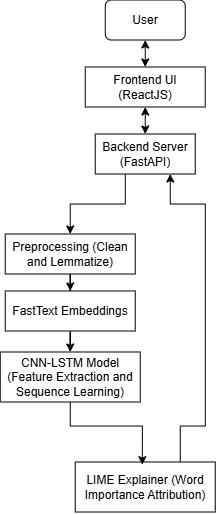
\includegraphics[height=0.48\textheight,keepaspectratio]{ArchitectureDiagram.drawio.png}
  \caption{System Architecture Diagram}
  \label{fig:architecture}
\end{figure}

\section{Data Flow Diagram Level 0}

The Data Flow Diagram Level 0, also designated as the context diagram, defines the
system boundary by illustrating the primary interactions between external entities
and the Ledger system as a single unified process.

Two principal external entities interact with the system: the User (or Fact-Checker)
and the Machine Learning Engineer (or System Administrator). The user submits unverified
news text or article headlines to the Ledger system. In return, the system provides
an authenticity assessment comprising the predicted label (Real or Fake), an associated
confidence percentage and word-level explainability highlights indicating the linguistic
basis for the prediction.

The machine learning engineer supplies annotated benchmark datasets, such as WELFake,
FakeNewsNet and LIAR, for offline model training and fine-tuning. The system outputs
training convergence metrics, cross-validation performance summaries and loss statistics
to allow the engineer to monitor model reliability.

\begin{figure}[H]
  \centering
  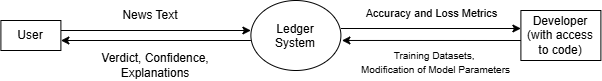
\includegraphics[width=0.92\textwidth,keepaspectratio]{DFD_0.drawio.png}
  \caption{Data Flow Diagram: Level 0 (Context Diagram)}
  \label{fig:dfd0}
\end{figure}

\section{Data Flow Diagram Level 1}

The Data Flow Diagram Level 1 decomposes the unified Ledger system into four modular
sub-processes, establishing the precise transformation of data from raw user input to
an explainable prediction.

Process 1.0 (Preprocess Text) receives raw text from the user and applies cleaning,
tokenization and lemmatization routines. Noise such as extraneous whitespace, HTML tags
and non-alphanumeric characters is removed to generate normalized token streams.

Process 2.0 (Generate Embeddings) takes the normalized tokens and retrieves corresponding
subword vector representations from the pre-trained FastText embedding repository. This
step ensures that out-of-vocabulary terms, typographical errors and internet slang are
projected into meaningful semantic vector spaces.

Process 3.0 (Classify News) feeds the dense embedding tensors into the trained CNN-LSTM
neural network. Pre-trained weights stored in the model repository evaluate local
syntactic patterns and sequential semantic flow, producing class probabilities for the
Real and Fake categories.

Process 4.0 (Generate Explanation) receives the prediction from the classification
process and invokes the LIME explainer. By perturbing words within the input sample and
fitting a localized linear surrogate model, the process calculates positive and negative
attribution weights for individual tokens. The final package, combining the veracity
verdict, confidence score and word-level attribution highlights, is transmitted back to
the user interface.

\begin{figure}[H]
  \centering
  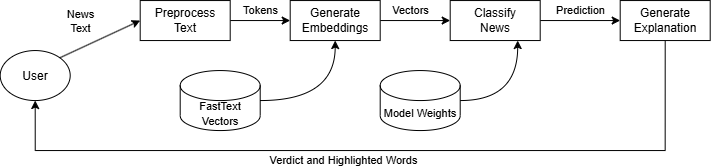
\includegraphics[width=0.92\textwidth,keepaspectratio]{DFD_1.drawio.png}
  \caption{Data Flow Diagram: Level 1}
  \label{fig:dfd1}
\end{figure}

\section{UML Sequence Diagram}

The UML Sequence Diagram illustrates the chronological message exchange between system
participants during a complete news verification lifecycle. The diagram models six
collaborating lifelines: the User, the React.js Frontend, the FastAPI Backend, the Text
Preprocessor and FastText Vectorizer, the CNN-LSTM Classifier and the LIME Explainer.

The sequence begins when the user submits news text and triggers the verification action
on the web interface. The React frontend sends an asynchronous HTTP POST request to the
FastAPI verification endpoint. The backend invokes the preprocessing and FastText
vectorizer module, which tokenizes the text and generates dense subword tensors before
returning them to the API handler.

The backend forwards the tensor representations to the CNN-LSTM classification model,
which computes the class likelihoods and returns the binary verdict alongside the
confidence percentage. To ensure transparency, the backend dispatches the input text
and model handle to the LIME explainer. LIME performs iterative word masking, queries
the model for surrogate inference on perturbed variants and calculates localized word
importance weights.

Once attribution weights are computed, LIME returns the attribution dictionary to the
backend. The FastAPI server packages the verdict, confidence score and word highlights
into a structured JSON payload and transmits it to the frontend client. The React
interface parses the payload and dynamically updates the dashboard, presenting the user
with a clear authenticity verdict and an interactive highlighted textual explanation.

\begin{figure}[H]
  \centering
  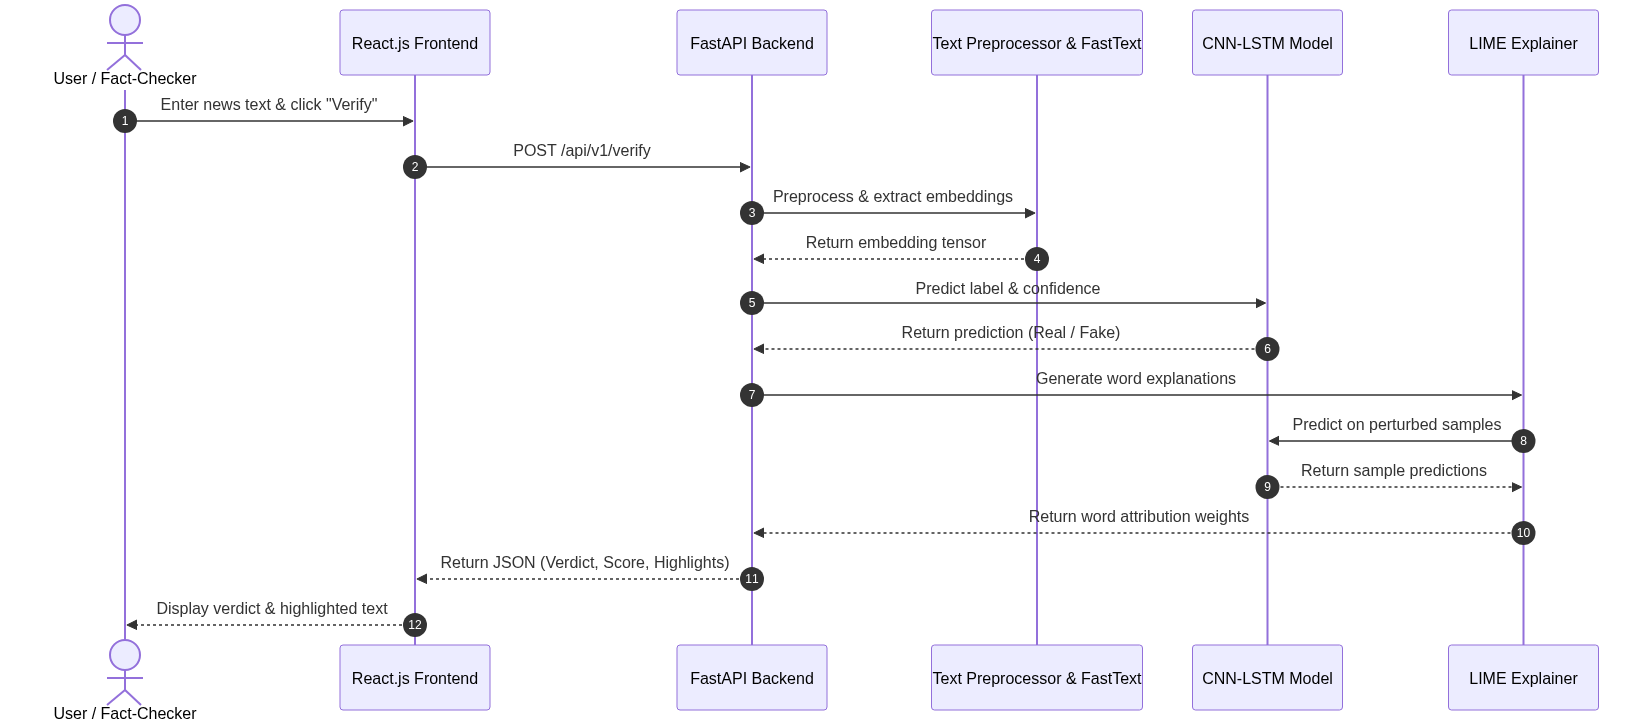
\includegraphics[width=0.95\textwidth,keepaspectratio]{uml_sequence_diagram.png}
  \caption{UML Sequence Diagram}
  \label{fig:sequence}
\end{figure}

%====================================================================
% REFERENCES
%====================================================================
\clearpage
\chapter*{REFERENCES}
\addcontentsline{toc}{chapter}{REFERENCES}
\markboth{REFERENCES}{REFERENCES}

\begin{enumerate}[label=\arabic*., leftmargin=*, itemsep=6pt]

  \item E. Hashmi, S. Y. Yayilgan, M. M. Yamin, S. Ali and M. Abomhara,
        ``Advancing Fake News Detection: Hybrid Deep Learning With FastText and
        Explainable AI,'' \textit{IEEE Access}, vol.~12, pp.~44463--44481, 2024.
        DOI: 10.1109/ACCESS.2024.3381038.

  \item P. K. Verma, P. Agrawal, I. Amorim and R. Prodan,
        ``WELFake: Word Embedding Over Linguistic Features for Fake News Detection,''
        \textit{IEEE Transactions on Computational Social Systems},
        vol.~8, no.~4, pp.~881--893, Aug. 2021.

  \item K. Shu, D. Mahudeswaran, S. Wang, D. Lee and H. Liu,
        ``FakeNewsNet: A Data Repository with News Content, Social Context and
        Spatiotemporal Information for Studying Fake News on Social Media,''
        \textit{Big Data}, vol.~8, no.~3, pp.~171--188, Jun. 2020.

  \item M. Umer, Z. Imtiaz, M. Ahmad, M. Nappi, C. Medaglia, G. S. Choi and
        A. Mehmood,
        ``Impact of Convolutional Neural Network and FastText Embedding on Text
        Classification,'' \textit{Multimedia Tools and Applications},
        vol.~82, no.~4, pp.~5569--5585, Feb. 2023.

  \item R. K. Kaliyar, A. Goswami and P. Narang,
        ``FakeBERT: Fake News Detection in Social Media using BERT and Deep
        Learning,'' \textit{Soft Computing}, vol.~25, no.~18,
        pp.~11771--11788, Sep. 2021.

  \item S. D. M. Kumar and A. M. Chacko,
        ``A Systematic Survey on Explainable AI Applied to Fake News Detection,''
        \textit{Engineering Applications of Artificial Intelligence},
        vol.~122, Art. no.~106087, Jun. 2023.

  \item K. Soga, S. Yoshida and M. Muneyasu,
        ``Exploiting Stance Similarity and Graph Neural Networks for Fake News
        Detection,'' \textit{Pattern Recognition Letters}, vol.~177,
        pp.~26--32, Jan. 2024.

  \item A. Altheneyan and A. Alhadlaq,
        ``Big Data ML-Based Fake News Detection Using Distributed Learning,''
        \textit{IEEE Access}, vol.~11, pp.~29447--29463, 2023.

  \item W. Y. Wang,
        ```Liar, Liar Pants on Fire': A New Benchmark Dataset for Fake News
        Detection,'' in \textit{Proc. 55th Annu. Meeting Assoc. Comput.
        Linguistics (ACL)}, 2017, pp.~422--426.

  \item J. A. Nasir, O. S. Khan and I. Varlamis,
        ``Fake news detection: A hybrid CNN-RNN based approach,''
        \textit{Int. J. Inf. Manage. Data Insights}, vol.~1, no.~2,
        Art. no.~100032, Nov. 2021.

  \item J. C. S. Reis, A. Correia, F. Murai, A. Veloso and F. Benevenuto,
        ``Supervised Learning for Fake News Detection: An Explainable Approach,''
        \textit{IEEE Internet Computing}, vol.~23, no.~2, pp.~46--53,
        Mar./Apr. 2019.

\end{enumerate}

\end{document}